% R4: Kernel PCA and hyperparameter tuning (Sanika). Numbers from scripts/run_baseline.py
% (kpca5 front-end), scripts/run_tuning.py and scripts/make_report_figures.py, seed 0.
% Needs: graphicx, booktabs. tab_tuning (18 rows) can move to an appendix if space is short.

\section{Kernel PCA and Hyperparameter Tuning}\label{sec:kpca}

\textbf{Kernel PCA.} To test whether a non-linear projection keeps the classes apart better
than PCA, we implemented RBF Kernel PCA by hand. We build the kernel matrix
$K_{ij}=\exp(-\gamma\lVert x_i-x_j\rVert^2)$, centre it in feature space, keep its top
eigenvectors, and project a new window through its centred kernel row. The kernel matrix
is $n\times n$, so it is fitted on at most 1,500 randomly chosen windows of the training
fold, while every window is projected. The default width is
$\gamma = 1/(d\,\mathrm{Var}(x)) = 1/126$ on standardised features, and we match the
bottleneck of PCA-5 and LDA-5 with $k=5$.

On clean data the non-linearity does not help (Fig.~\ref{fig:kpca}, left). Held-out
Fisher $J$ of Kernel PCA tracks linear PCA up to $k=4$ and falls behind at $k=5$ (12.0
against 16.1 for PCA and 16.2 for LDA). The best classifier on Kernel PCA-5 reaches a
grouped macro-F1 of 0.35 (linear SVM), against 0.39 for PCA-5, 0.45 for the raw features
and 0.49 for LDA-5 with a random forest. That 0.35 is a favourable draw of the
1,500-window subsample: with four other subsample seeds the same model scores 0.26--0.31,
and exact Kernel PCA on all training windows scores 0.31. Nested tuning (below) most often
picks a \emph{wider} kernel, $\gamma=0.002$, which moves Kernel PCA closer to linear PCA.
It is the most frequent choice for 4 of the 6 classifiers, but each of those wins only 2--3
of the 6 folds.
% TODO(1c): Kernel PCA-5 under corruption (the original motivation for a non-linear
% front-end) goes here once the multi-seed corruption sweeps have been run.

\begin{figure*}[t]
  \centering
  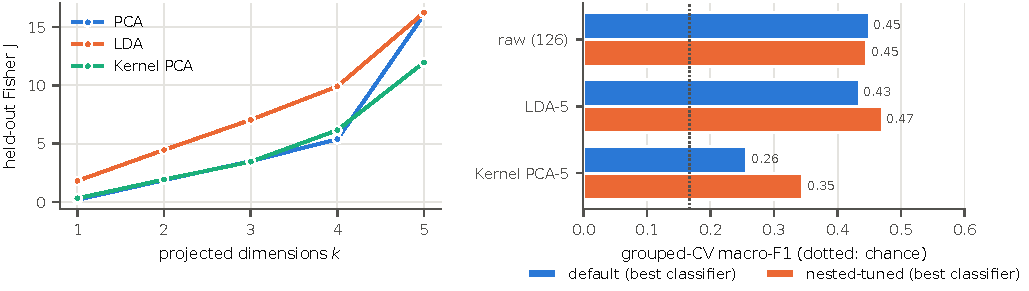
\includegraphics[width=\textwidth]{figures/fig_kpca.pdf}
  \caption{Left: held-out Fisher $J$ against the number of projected dimensions.
  Right: grouped-CV macro-F1 of the best classifier per front-end, with fixed defaults and
  after nested tuning; dotted line: chance (1/6). Both bars fit on every second training
  window, so the defaults sit below the baseline scores quoted in the text.}
  \label{fig:kpca}
\end{figure*}

\textbf{Nested tuning.} The baseline uses fixed hyperparameters ($k=5$ neighbours, SVM
$C=1$ or 10, 300 fully grown trees). To check whether these limit accuracy, we tuned every
classifier on the raw, LDA-5 and Kernel PCA-5 front-ends without selection bias. The outer
loop is the usual six grouped folds. Inside each outer training fold, the five remaining
recordings per class form five inner grouped folds, and a grid search (neighbours
$\{1,5,15,45\}$; linear $C\in\{0.01,0.1,1,10\}$; RBF $C\in\{1,10,100\}$ and
$\gamma$; forest minimum leaf size $\{1,10\}$; Naive Bayes variance smoothing; and the
Kernel PCA $\gamma\in\{0.002, 1/126, 0.03\}$) picks the setting with the best inner
macro-F1. That setting is refit on the outer training fold and scored once on the outer
test recordings. To keep the search affordable, fits use every second window of each
training recording (neighbouring windows overlap by 50\%), for both the tuned and the
default models. The default scores here are therefore not the baseline scores above.
Halving the training windows lowers LDA-5 with a random forest from 0.49 to 0.43, and which
half is used moves it by up to 0.03. Kernel PCA-5 with a linear SVM drops from 0.35 to
0.26, which is within its subsample-to-subsample spread.

Tuning changes little (Table~\ref{tab:tuning}). On the raw and LDA-5 front-ends the gain
over the defaults lies between $-0.03$ and $+0.04$ macro-F1, well inside the fold-to-fold
spread of 0.10--0.17, and the best model stays LDA-5 with a random forest (0.47 tuned,
0.43 default). The largest gain is for Kernel PCA-5 with an RBF SVM (0.22 to 0.35), but
even tuned, Kernel PCA stays below the linear front-ends. The selected settings are also
unstable: the most frequent choice wins only 2--6 of the 6 outer folds, and only 2--3 for
Kernel PCA. The fixed defaults are therefore not what limits accuracy. The limit is the
shift from one recording to the next, since each class is recorded only once per
condition.

\begin{table}[t]
  \centering
  \caption{Nested grouped tuning: macro-F1 with fixed defaults and after tuning (mean of
  6 outer folds), and the most frequently selected setting (folds it won). Both columns fit
  on every second training window, so the defaults sit below the baseline scores.}
  \label{tab:tuning}
  \resizebox{\columnwidth}{!}{\begin{tabular}{llrrrl}
\toprule
Front & Classifier & default & tuned & gain & most chosen (folds) \\
\midrule
raw & knn\_euc & 0.30 & 0.28 & -0.02 & n\_neighbors=1 (3/6) \\
raw & knn\_mah & 0.28 & 0.31 & +0.03 & n\_neighbors=45 (6/6) \\
raw & svm\_lin & 0.45 & 0.45 & +0.00 & C=0.1 (3/6) \\
raw & svm\_rbf & 0.37 & 0.37 & +0.00 & C=1.0, gamma=scale (6/6) \\
raw & rf & 0.40 & 0.37 & -0.03 & min\_samples\_leaf=1 (5/6) \\
raw & gnb & 0.27 & 0.28 & +0.01 & var\_smoothing=0.1 (5/6) \\
lda5 & knn\_euc & 0.41 & 0.42 & +0.01 & n\_neighbors=1 (5/6) \\
lda5 & knn\_mah & 0.40 & 0.41 & +0.01 & n\_neighbors=1 (3/6) \\
lda5 & svm\_lin & 0.43 & 0.43 & +0.00 & C=0.1 (4/6) \\
lda5 & svm\_rbf & 0.41 & 0.40 & -0.01 & C=10.0, gamma=scale (4/6) \\
lda5 & rf & 0.43 & 0.47 & +0.04 & min\_samples\_leaf=10 (3/6) \\
lda5 & gnb & 0.40 & 0.41 & +0.01 & var\_smoothing=0.001 (3/6) \\
kpca5 & knn\_euc & 0.17 & 0.22 & +0.05 & n\_neighbors=5, kpca\_gamma=0.002 (2/6) \\
kpca5 & knn\_mah & 0.18 & 0.18 & +0.00 & n\_neighbors=1, kpca\_gamma=scale (2/6) \\
kpca5 & svm\_lin & 0.26 & 0.28 & +0.02 & C=10.0, kpca\_gamma=scale (3/6) \\
kpca5 & svm\_rbf & 0.22 & 0.35 & +0.13 & C=10.0, gamma=scale, kpca\_gamma=0.002 (2/6) \\
kpca5 & rf & 0.20 & 0.21 & +0.01 & min\_samples\_leaf=1, kpca\_gamma=0.002 (3/6) \\
kpca5 & gnb & 0.22 & 0.24 & +0.02 & var\_smoothing=0.1, kpca\_gamma=0.002 (2/6) \\
\bottomrule
\end{tabular}
}
\end{table}
